\documentclass[a4paper]{article}
\usepackage[utf8x]{inputenc}
\usepackage[T1,T2A]{fontenc}
\usepackage[russian]{babel}
\usepackage{hyperref}
\usepackage{indentfirst}
\usepackage{listings}
\usepackage{color}
\usepackage{here}
\usepackage{array}
\usepackage{multirow}
\usepackage{graphicx}
\usepackage{amsmath} 
\usepackage{spverbatim}

\usepackage{caption}
\renewcommand{\lstlistingname}{Программа} % заголовок листингов кода


\lstset{ %
	extendedchars=\true,
	keepspaces=true,
	language=bash,					% choose the language of the code
	basicstyle=\footnotesize,		% the size of the fonts that are used for the code
	numbers=left,					% where to put the line-numbers
	numberstyle=\footnotesize,		% the size of the fonts that are used for the line-numbers
	stepnumber=1,					% the step between two line-numbers. If it is 1 each line will be numbered
	numbersep=5pt,					% how far the line-numbers are from the code
	backgroundcolor=\color{white},	% choose the background color. You must add \usepackage{color}
	showspaces=false				% show spaces adding particular underscores
	showstringspaces=false,			% underline spaces within strings
	showtabs=false,					% show tabs within strings adding particular underscores
	frame=single,           		% adds a frame around the code
	tabsize=2,						% sets default tabsize to 2 spaces
	captionpos=b,					% sets the caption-position to bottom
	breaklines=true,				% sets automatic line breaking
	breakatwhitespace=false,		% sets if automatic breaks should only happen at whitespace
	escapeinside={\%*}{*)},			% if you want to add a comment within your code
	postbreak=\raisebox{0ex}[0ex][0ex]{\ensuremath{\color{red}\hookrightarrow\space}}
}

\usepackage[left=2cm,right=2cm,
top=2cm,bottom=2cm,bindingoffset=0cm]{geometry}

\begin{document}	% начало документа

\begin{titlepage}	% начало титульной страницы

	\begin{center}		% выравнивание по центру

		\largeФедеральное государственное автономное образовательное учреждение высшего образования «Санкт-Петербургский политехнический университет Петра Великого» \\
		\large Институт компьютерных наук и технологий \\
		\large Кафедра компьютерных систем и программных технологий\\[2cm]
		% название института, затем отступ 6см
		
	    \vfill
		\hugeТелекоммуникационные технологии\\[0.5cm] % название работы, затем отступ 0,5см
		\large Лабораторная работа №3:\\
		Линейная фильтрация\\[4.8cm]

	\end{center}

	\begin{flushright} % выравнивание по правому краю
		\begin{minipage}{0.25\textwidth} % врезка в половину ширины текста
			\begin{flushleft} % выровнять её содержимое по левому краю

				\large\textbf{Работу выполнил:}\\
				\large Сергеев ~А.А.\\
				\large {Группа:} 33531/2\\
				
				\large \textbf{Преподаватель:}\\
				\large Богач ~Н.В.\\

			\end{flushleft}
		\end{minipage}
	\end{flushright}
	
	\vfill % заполнить всё доступное ниже пространство

	\begin{center}
	\large Санкт-Петербург\\
	\large \the\year % вывести дату
	\end{center} % закончить выравнивание по центру

\thispagestyle{empty} % не нумеровать страницу
\end{titlepage} % конец титульной страницы
\vfill % заполнить всё доступное ниже пространство

% Содержание
\tableofcontents

\newpage
\section{Цель работы}
Изучить воздействие ФНЧ на тестовый сигнал с шумом.
\section{Постановка задачи}
Сгенерировать гармонический сигнал с шумом и синтезировать ФНЧ. Получить сигнал во временной и частотной областях до и после фильтрации. Сделать выводы о воздействии ФНЧ на спектр сигнала.
\section{Теоретический раздел}
\subsection{Сущность линейной дискретной обработки}
Линейный дискретный фильтр -- это произвольная система обработки сигнала, обладающая свойствами линейности и стационарности.
\begin{itemize}
    \item Линейность означает, что выходная реакция на сумму воздействий равна сумме реакций на эти воздействия, поданные на вход по отдельности.
    \item Стационарность означает, что задержка входного сигнала приводит лишь к такой же задержке выходного сигнала, не меняя его формы.
\end{itemize}
В общем случае дискретный фильтр суммирует (с весовыми коэффициентами) неко- торое количество входных отсчетов (включая последний) и некоторое количество предыдущих выходных отсчетов:
$$y(k)=b_0x(k)+b_1x(k−1)+b_2x(k−2)+...+b_mx(k−m)−a_1y(k−1)−a_2y(k−2)−...−a_ny(k−n)$$
где $a_j$, $b_i$ -- вещественные коэффициенты.\\
Вышеприведенная формула называется алгоритмом или уравнением дискретной фильтрации. Если сгруппировать слагаемые так, чтобы с одной строны от знака равенства были только входные отсчеты, а с другой -- только выходные, получим форму записи, называемую разностным уравнением:
$$y(k)+a_1y(k−1)+a_2y(k−2)+...+a_ny(k−n)=b_0x(k)+b_1x(k−1)+b_2x(k−2)+...+b_mx(k−m)$$
\subsection{Описание дискретных систем}
В случае линейных систем с постоянными параметрами для анализа прохождения любого сигнала достаточно знать результат прохождения элементарного импульса в виде $\delta$-функции. Для дискретных систем вместо $\delta$-функции рассматривают единичную импульсную функцию $x_0(k)$:\\
\begin{equation*}
    x_0(k)= \begin{cases}
                $1$, & $k=0$\\
                $0$, & $k\ne0$\\
            \end{cases}
\end{equation*}

Реакция дискретной системы на единичный импульс $x_0(k)$ называется импульсной характеристикой этой системы и обозначается $h(k)$.\\
Для физически реализуемой системы $h(k)=0$ при $k<0$, поэтому выходной сигнал дискретной линейной стационарной системы выражается через входной как
$$y(k)=\sum_{m=-\infty}^{k}x(m)h(k-m)=\sum_{m=0}^{\infty}x(k-m)h(m)$$

Это означает, что система при вычислении очередного отсчета может оперировать только прошлыми значениями входного сигнала и еще ничего не знает о будущих. С математической точки зрения данная формула представляет собой дискретную линейную свертку входного сигнала с импульсной характеристикой системы, через которую проходит этот сигнал.
\subsection{Функция передачи}
Свертке сигналов во временной области соответствует произведение их спектров в частотной. При анализе дискретных сигналов используют так называемое $z$-преобразование, свойства которого аналогичны преобразованиям Фурье и Лапласа. Поэтому дискретной свертке $x(k)$ и $h(k)$ будет соответствовать произведение $z$-преобразований этих последовательностей:\\
$Y(z)=H(z)X(z)$,\\
где $H(z)$ -- функция передачи (transfer function) или системная функция:
$$H(z)=\frac{Y(z)}{X(z)}=\sum_{k=0}^{\infty}h(k)z^{-k}$$
\subsection{Частотная характеристика}
Если подставить в функцию передачи $e^{j\omega T}$(здесь $T$ -- период дискретизации) в качестве аргумента, получим частотную характеристику дискретной системы:
$$\dot{K}(\omega)=H(e^{j\omega t})=\sum_{k=0}^{\infty}h(k)e^{-j\omega kT}$$

\subsection{Нерекурсивные фильтры}
Нерекурсивными называют фильтры, которые не используют предыдущие отсчеты выходного сигнала при вычислении следующих. Для них уравнение фильтрации упрощается и принимает вид:
$$y(k)=\sum_{i=0}Kb_ix(k − i)$$
Количество $K$ используемых отсчетов входного сигнала называется порядком фильтра. Структурная схема, реализующая алгоритм, приведена на рис. 1. Блоки, подписанные как <<$z^{-1}$>>, соответствуют задержке входного сигнала на $1$ такт (что равносильно умножению $z$-преобразования задерживаемой последовательности на $z^{-1}$).\\

Импульсная характеристика нерекурсивного фильтра определяется путем подстановки в уравнение единичного импульса $x_0(k)$ в качестве входного сигнала:
$$h(k)=\sum_{i=0}Kb_ix_0(k − i) = b_k$$
так как $x_0(k - i)\ne0$ только для $i=k$.

Таким образом, коэффициенты $b_i$ нерекурсивного фильтра являются отсчетами его импульсной характеристики. Так как в реальном устройстве линия задержки содержит конечное число элементов, то импульсная характеристика нерекурсивного фильтра также является конечной по длительности.\\
Поэтому еще одно название таких фильтров -- фильтры с конечной импульсной характеристикой (КИХ-фильтры, английский термин -- finite impulse response, FIR).

\subsection{Рекурсивные фильтры}
Если уравнение фильтрации содержит как входные, так и выходные отсчеты, то для реализации такого фильтра необходимо добавить вторую линию задержки -- для хранения выходных отсчетов $y(k - i)$.

Так как при вычислениях используются предыдущие отсчеты выходного сигнала, в
схеме присутствуют обратные связи. Поэтому такие фильтры называют рекурсивными. Для таких фильтров уравнение фильтрации может быть записано следующим образом:
$$y(k)=\sum_{i=0}Kb_ix(k − i)-\sum_{i=1}Na_iy(k − i)$$
где $max(K,N)$ называют порядком данного рекурсивного фильтра.

Так как каждый следующий отсчет импульсной характеристики рекурсивного фильтра вычисляется исходя из значения предыдущего, то количество таких отсчетов не ограничено. Поэтому рекурсивные фильтры называют также фильтрами с бесконечной импульсной характеристикой (БИХфильтрами, английский термин -- infinite impulse response, IIR). По этой же причине рекурсивные фильтры могут быть неустойчивыми.
\newpage
\section{Ход работы}
Для демонстрации работы фильтров используем сигналы из лабораторной работы 1. 
\subsection{Синусоидальный сигнал}\\
\subsubsection{Синусоидальынй сигнал и его спектр}
\lstinputlisting[language=Matlab]{lab3/sin/sin_sig.m}\\
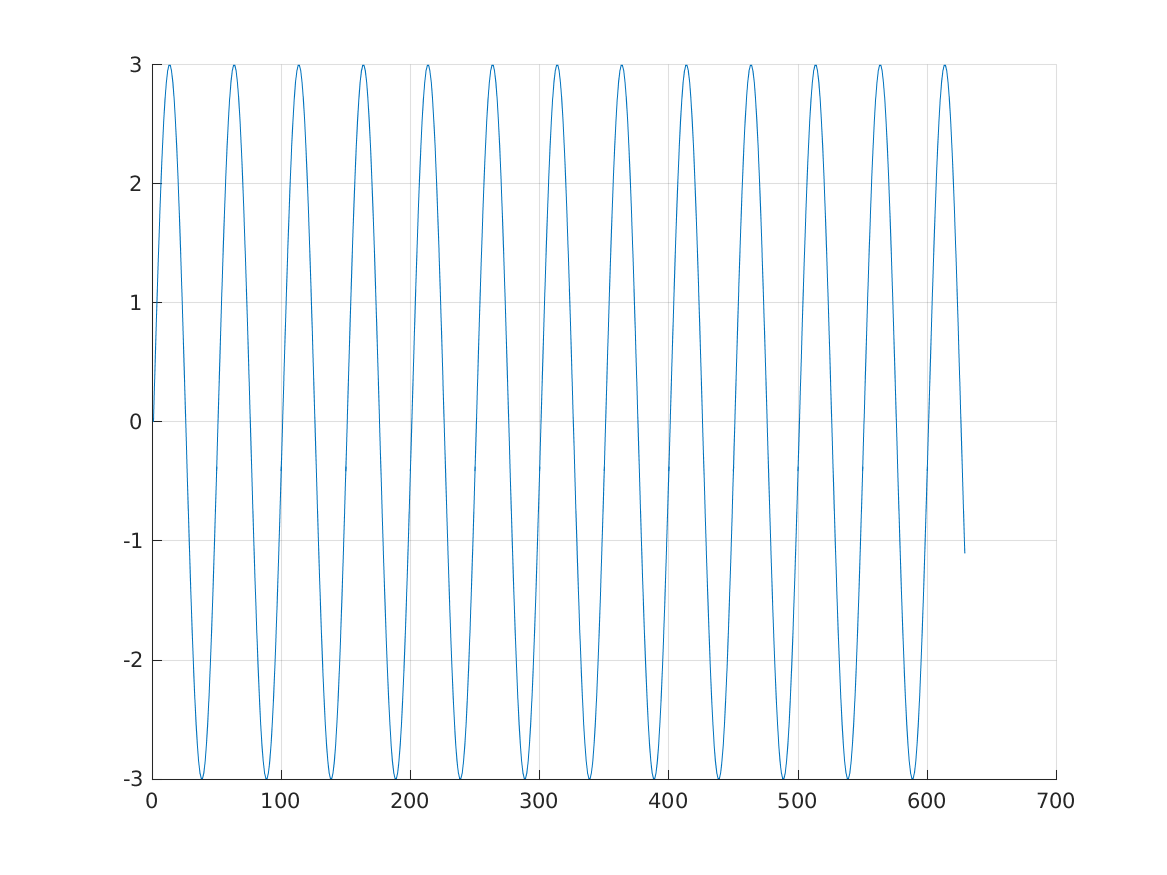
\includegraphics[scale=0.7]{lab3/figures/figure_0.png}\\
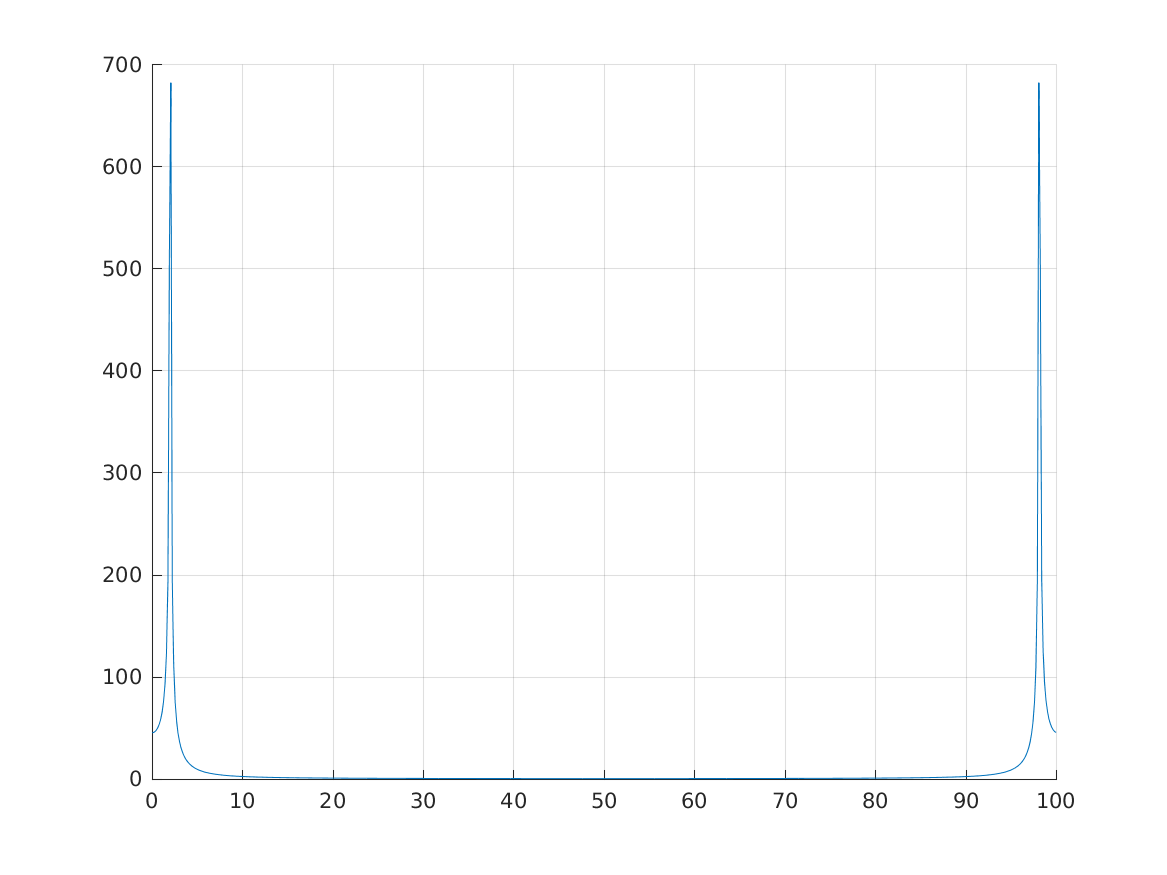
\includegraphics[scale=0.7]{lab3/figures/figure_1.png}\\
\subsubsection{Зашумленный синусоидальный сигнал и его спектр}\\
\lstinputlisting[language=Matlab]{lab3/sin/noise_sin_sig.m}\\
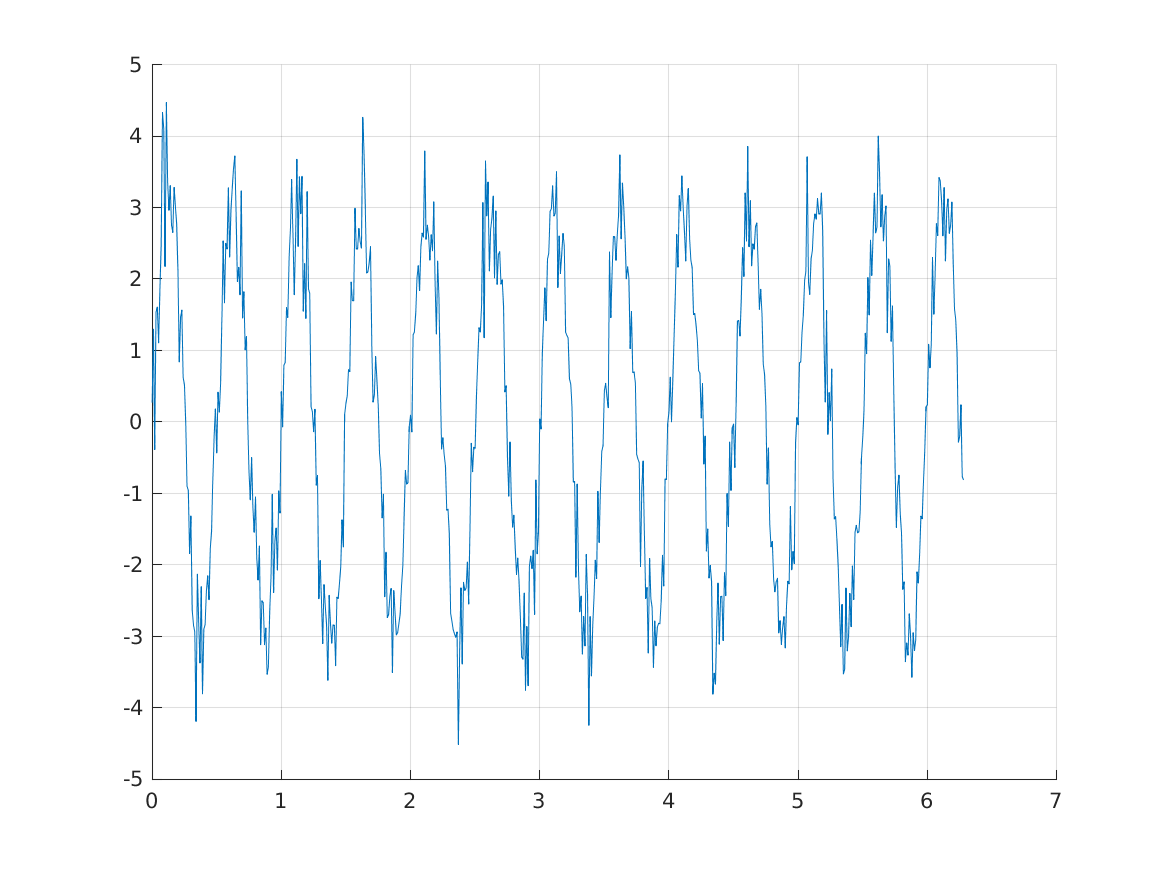
\includegraphics[scale=0.7]{lab3/figures/figure_2.png}\\
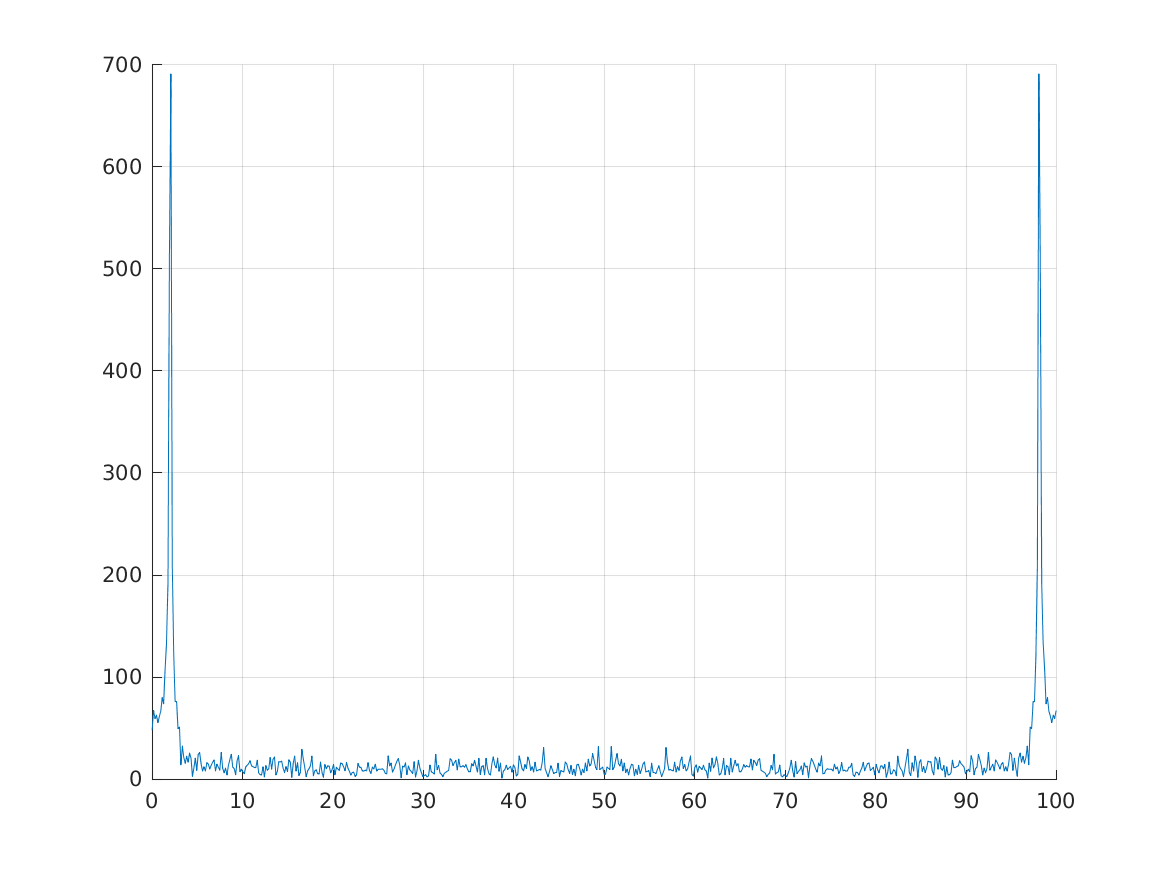
\includegraphics[scale=0.7]{lab3/figures/figure_3.png}\\
\subsubsection{Применение фильтра}\\
Релизация фильтра и его настройка:\\
\newpage
\lstinputlisting[language=Matlab]{lab3/filter.m}\\
Фильтрация сигнала:\\
\lstinputlisting[language=Matlab]{lab3/sin/filter_sin_sig.m}\\
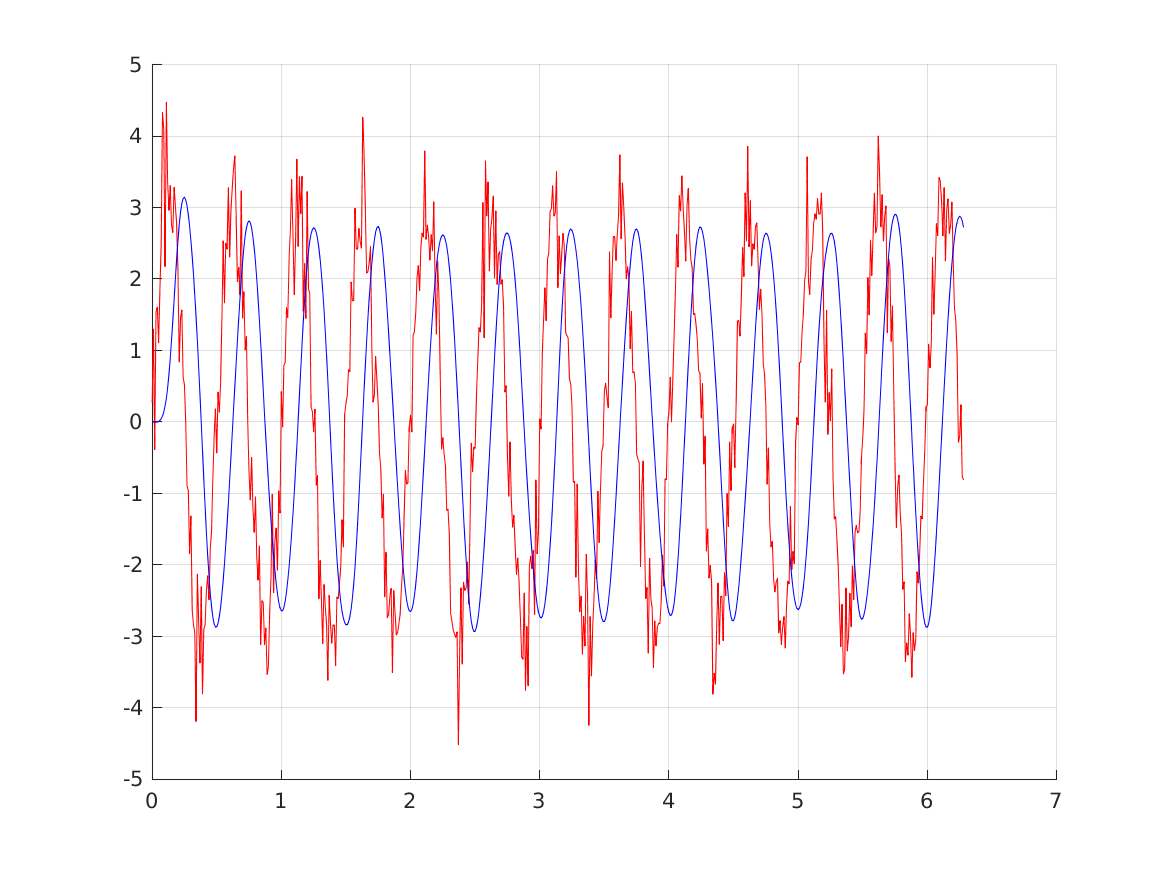
\includegraphics[scale=0.7]{lab3/figures/figure_4.png}\\
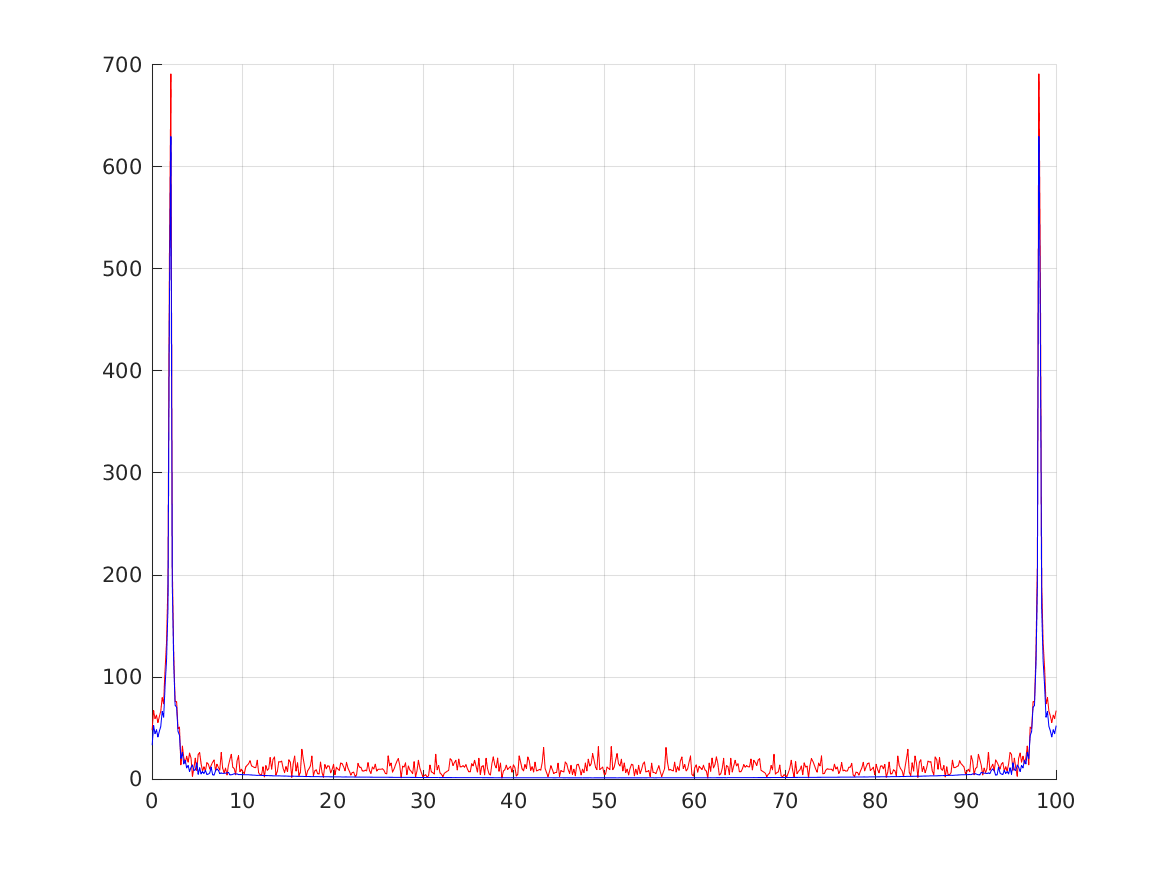
\includegraphics[scale=0.7]{lab3/figures/figure_5.png}\\
\subsection{Прямоугольный сигнал}\\
\subsubsection{Прямоугольный сигнал и его спектр}\\
\lstinputlisting[language=Matlab]{lab3/square/square_sig.m}\\
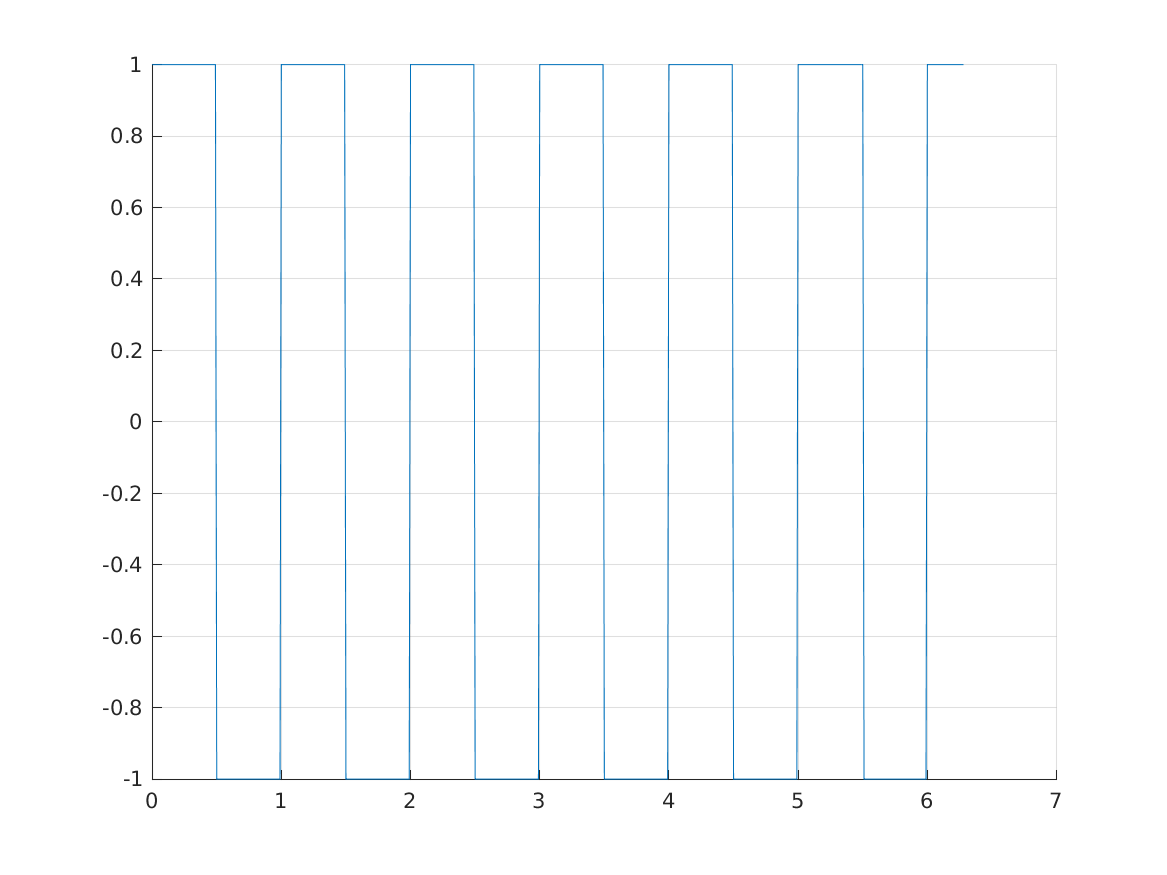
\includegraphics[scale=0.7]{lab3/figures/figure_6.png}\\
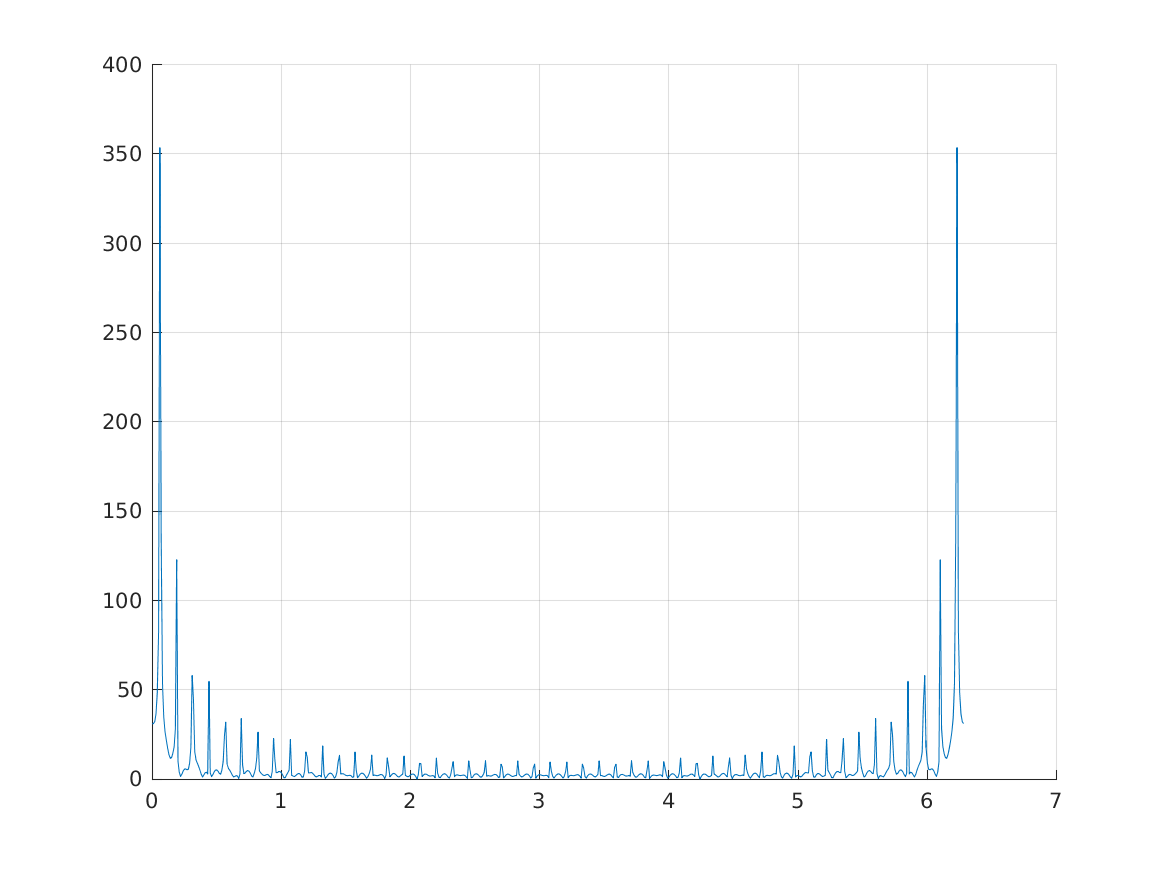
\includegraphics[scale=0.7]{lab3/figures/figure_7.png}\\
\subsubsection{Зашумленный прямоугольный сигнал и его спектр}\\
\newpage
\lstinputlisting[language=Matlab]{lab3/square/noise_square_sig.m}\\
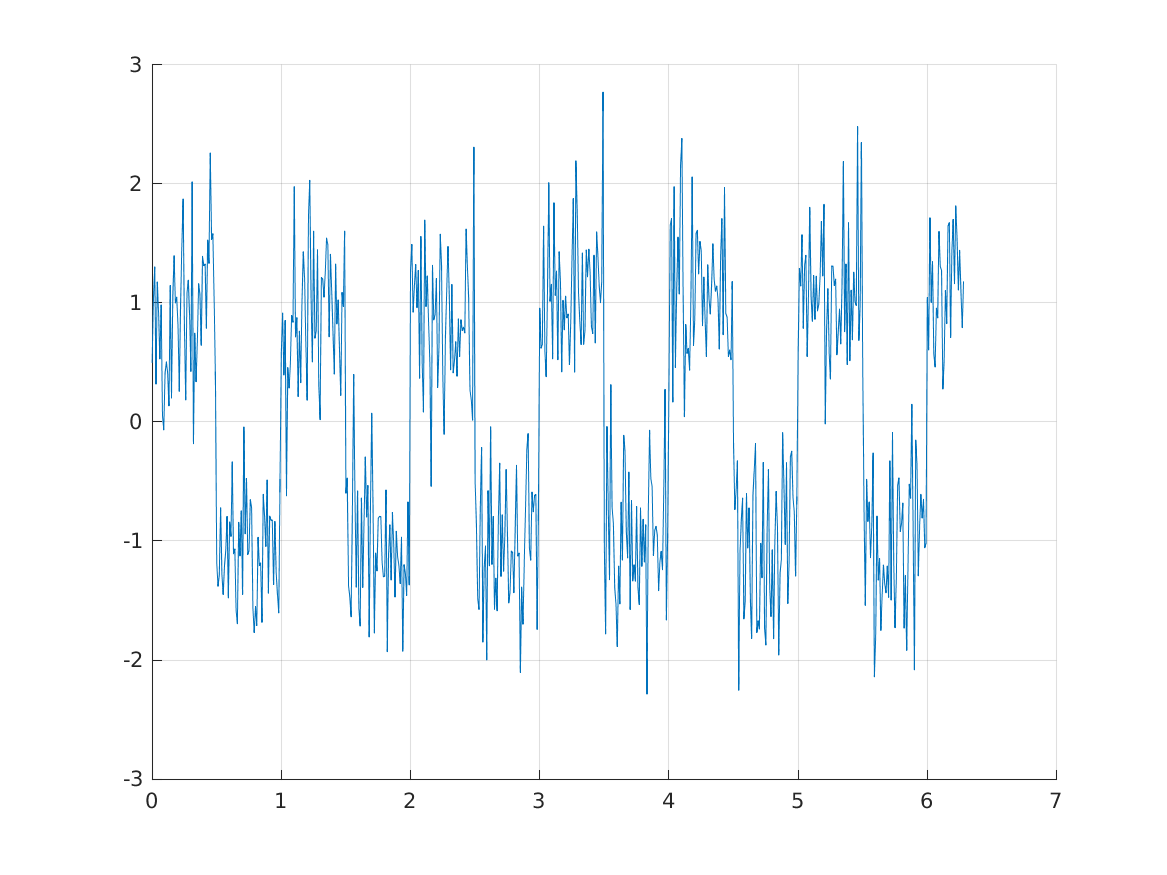
\includegraphics[scale=0.7]{lab3/figures/figure_8.png}\\
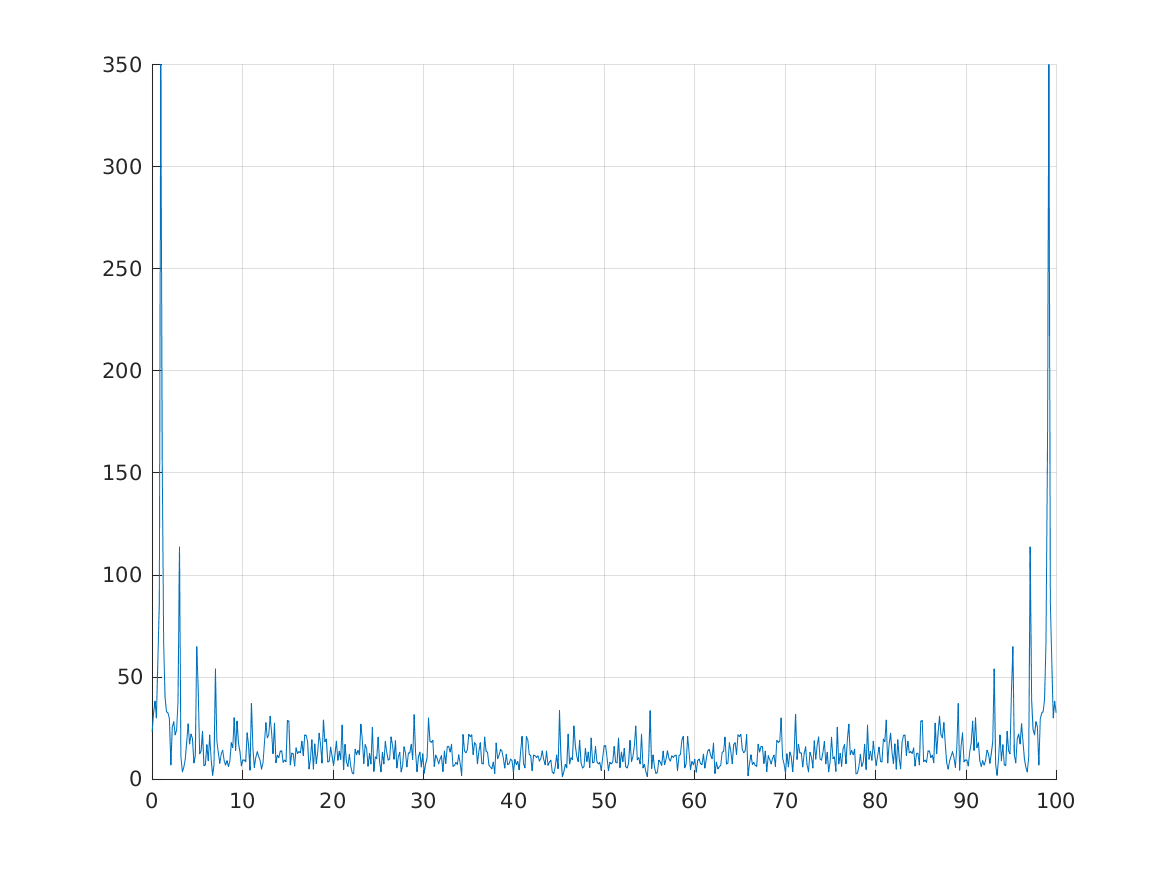
\includegraphics[scale=0.7]{lab3/figures/figure_9.png}\\
\subsubsection{Применение фильтра}\\
Релизация фильтра и его настройка:\\
\lstinputlisting[language=Matlab]{lab3/filter.m}\\
Фильтрация сигнала:\\
\lstinputlisting[language=Matlab]{lab3/square/filter_square_sig.m}\\
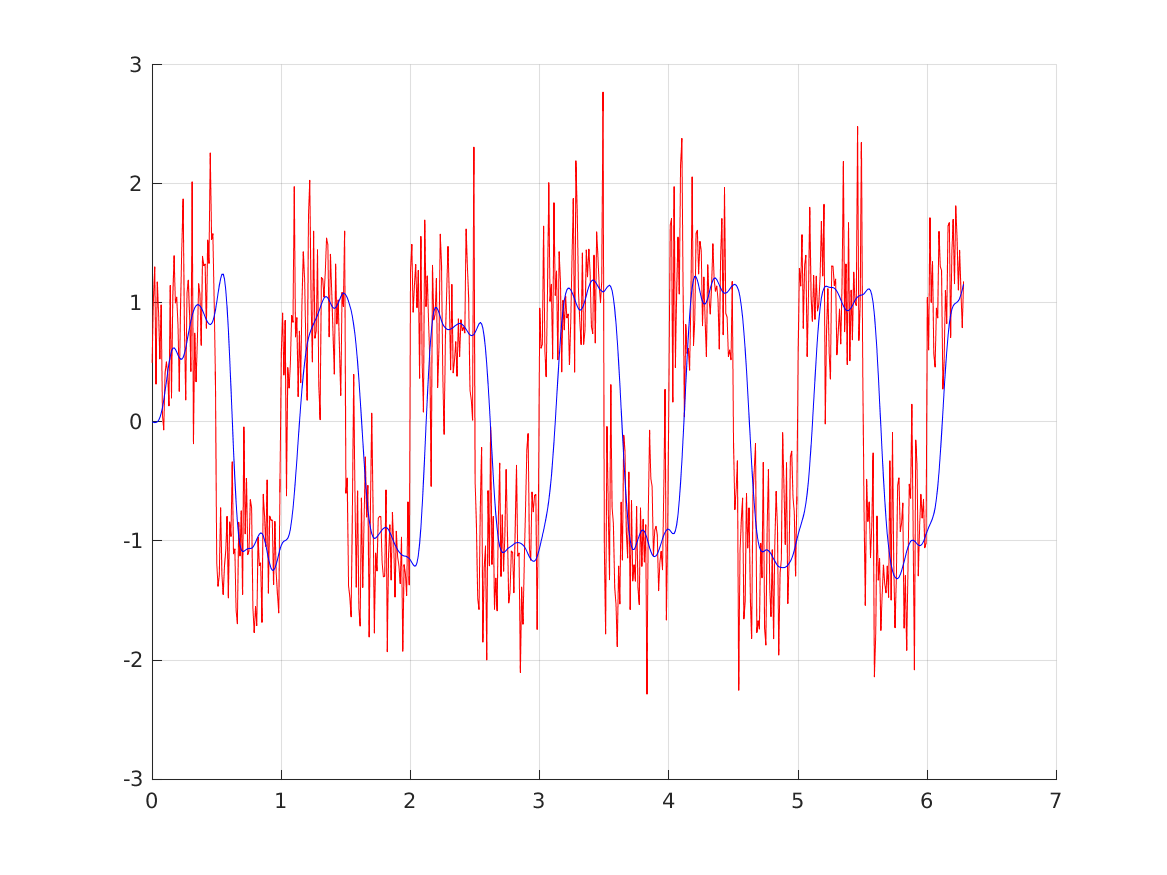
\includegraphics[scale=0.7]{lab3/figures/figure_10.png}\\
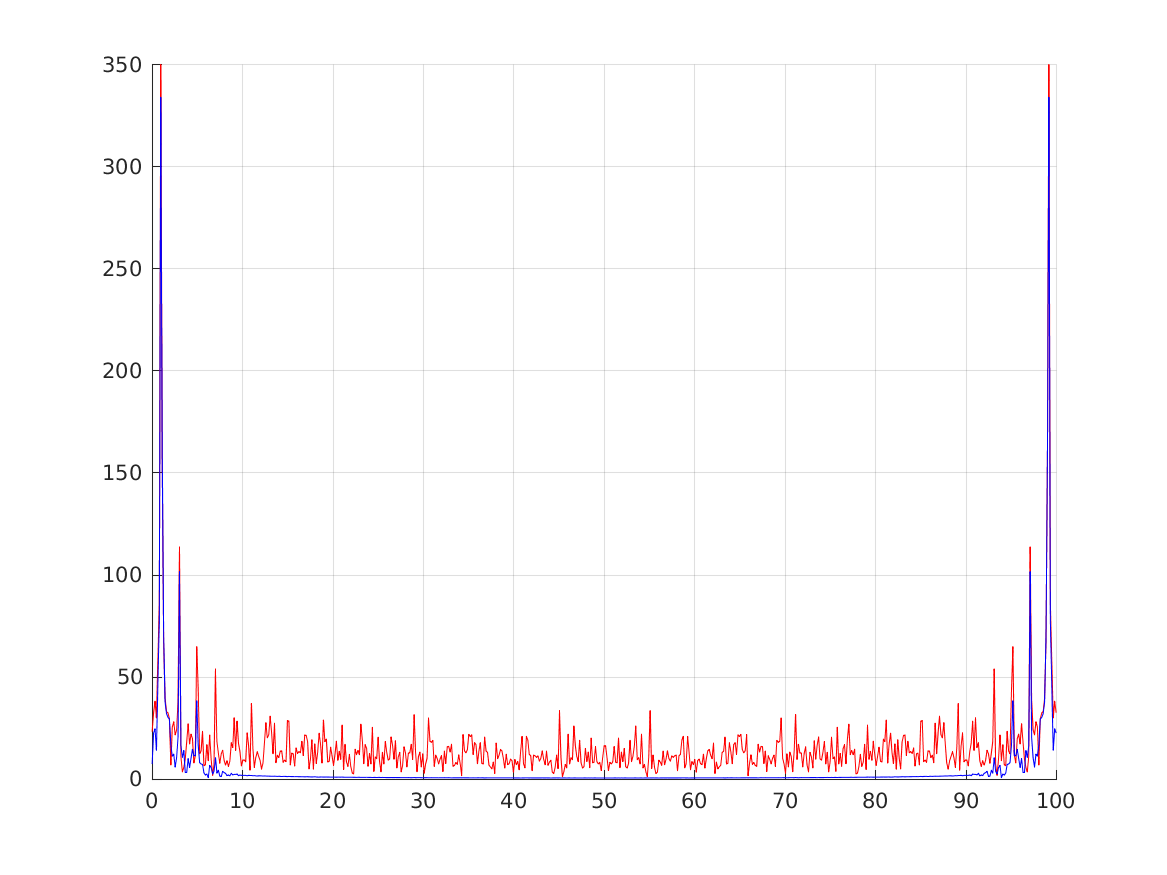
\includegraphics[scale=0.7]{lab3/figures/figure_11.png}\\
\subsection{Треугольный сигнал}\\
\subsubsection{Треугольынй сигнал и его спектр}\\
\lstinputlisting[language=Matlab]{lab3/triangle/triangle_sig.m}\\
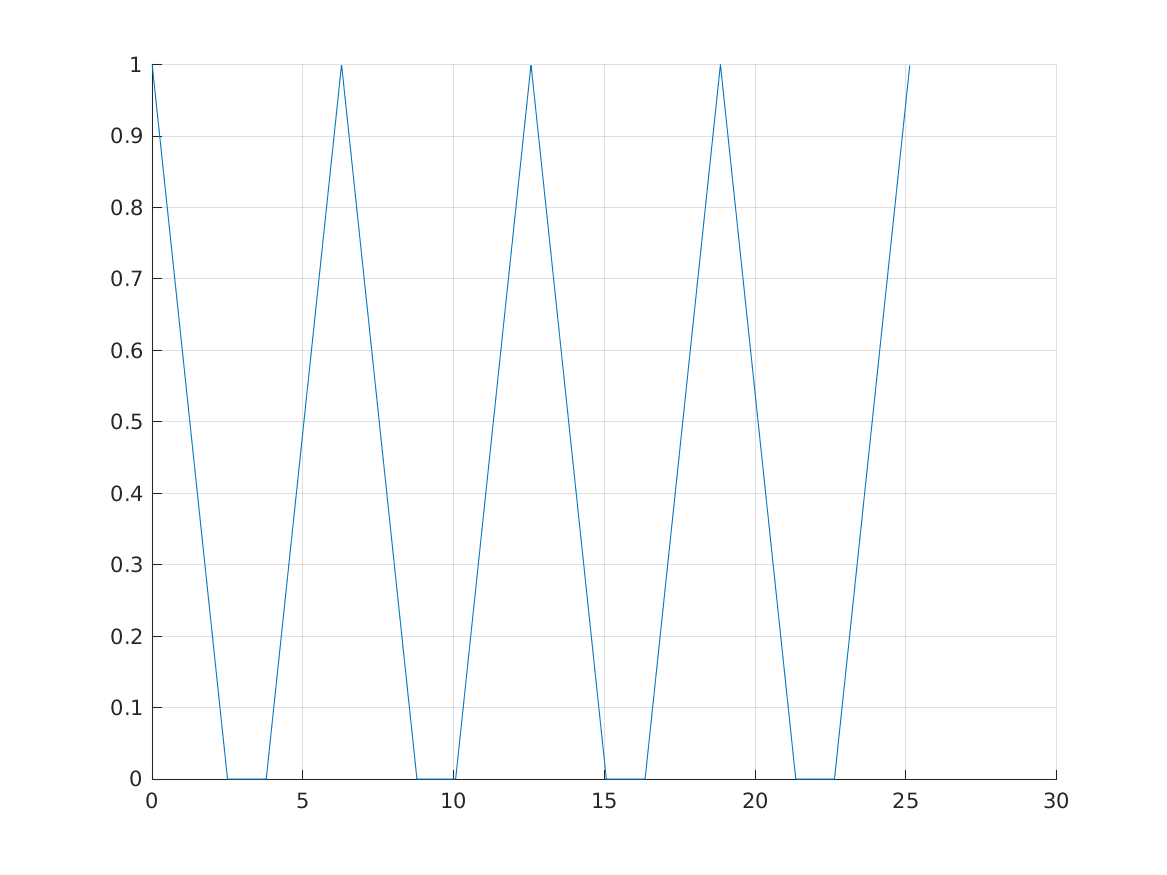
\includegraphics[scale=0.7]{lab3/figures/figure_12.png}\\
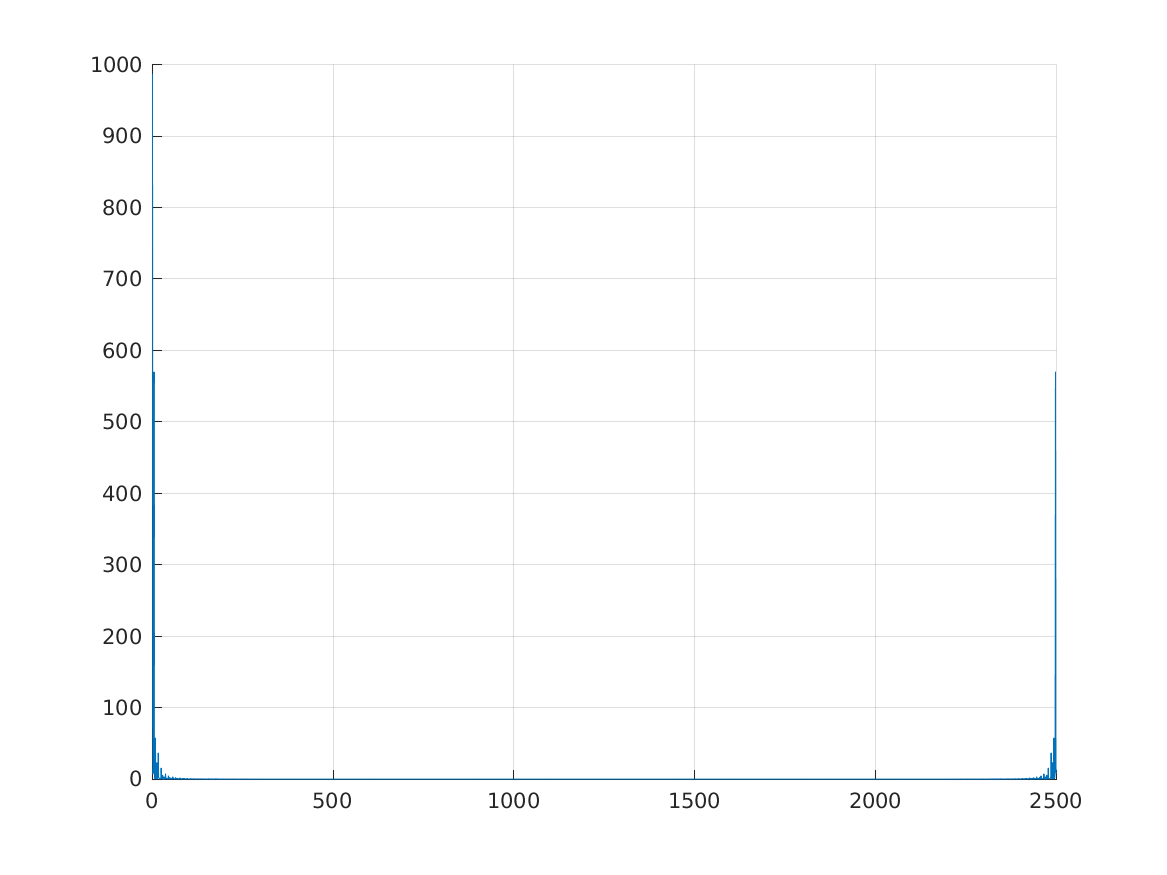
\includegraphics[scale=0.7]{lab3/figures/figure_13.png}\\
\subsubsection{Зашумленный треугольный сигнал и его спектр}\\
\lstinputlisting[language=Matlab]{lab3/triangle/noise_triangle_sig.m}\\
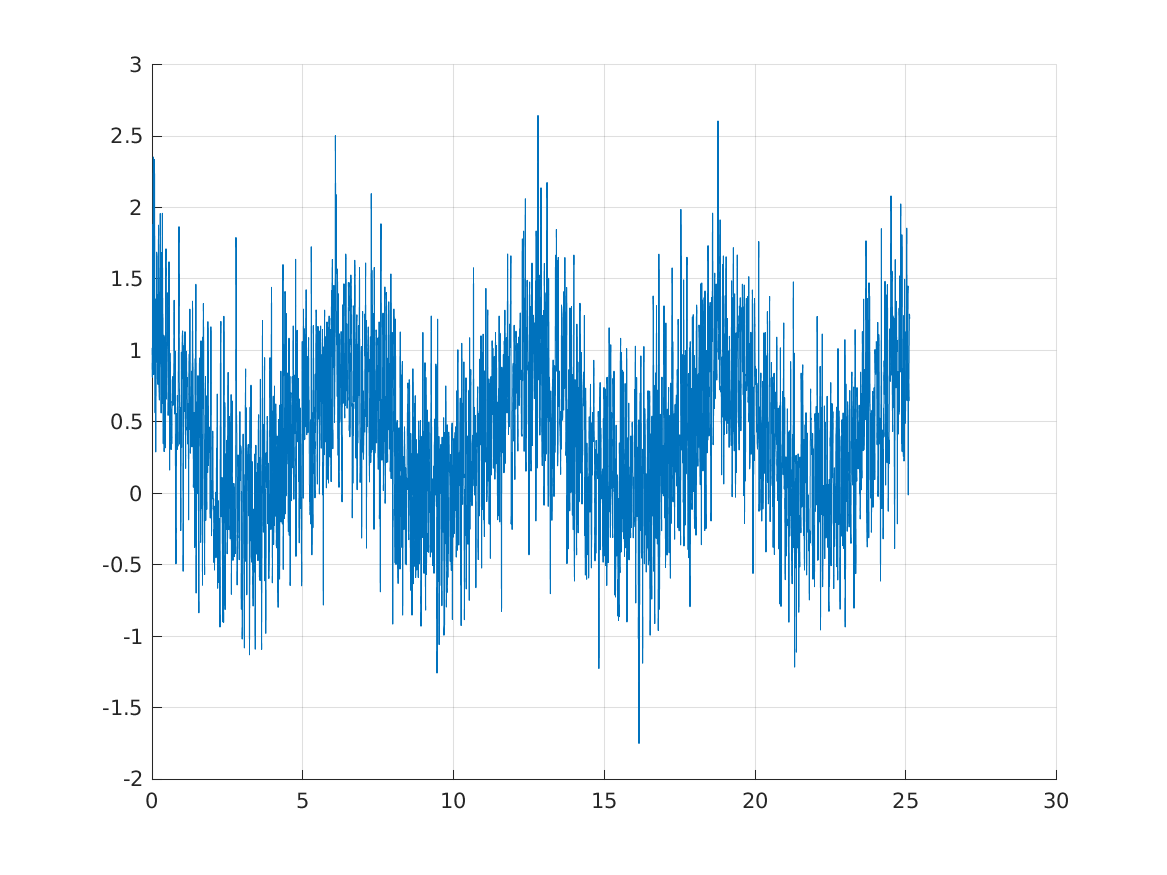
\includegraphics[scale=0.7]{lab3/figures/figure_14.png}\\
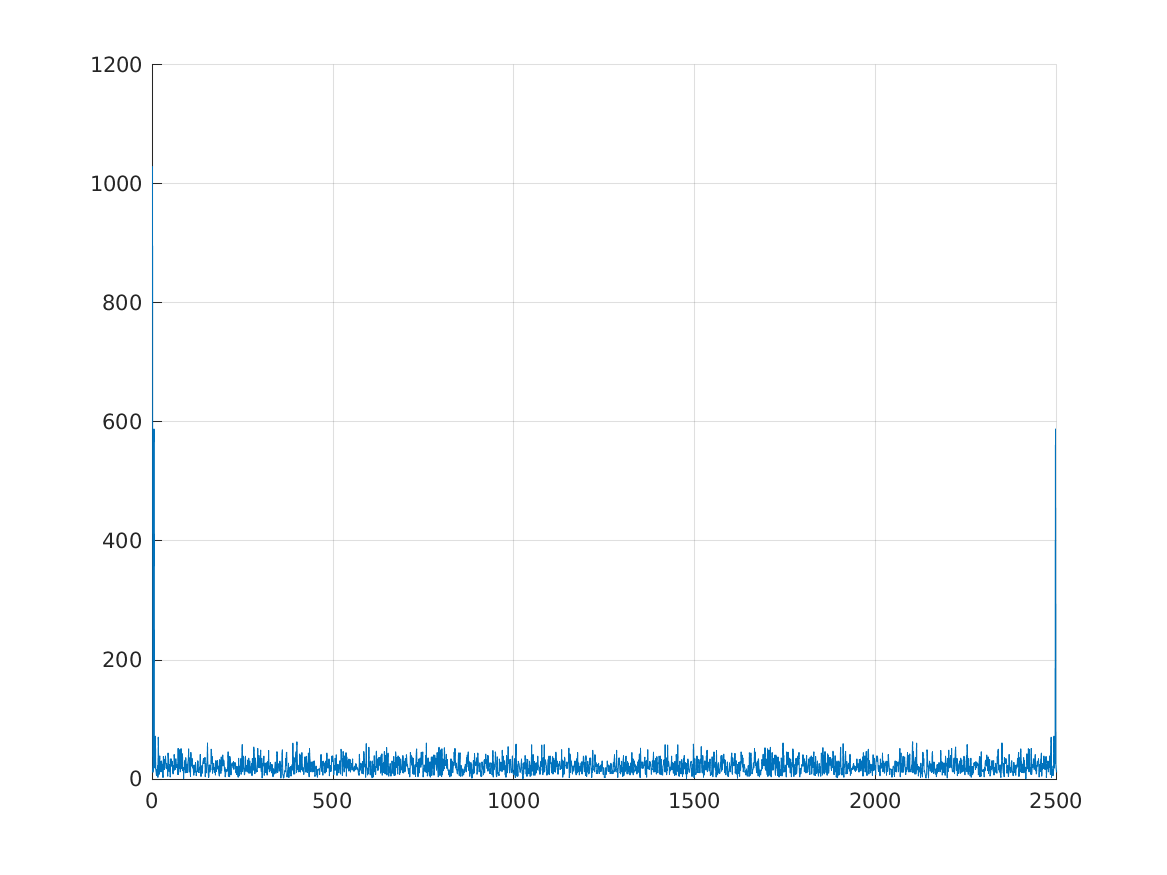
\includegraphics[scale=0.7]{lab3/figures/figure_15.png}\\
\subsubsection{Применение фильтра}\\
Релизация фильтра и его настройка:\\
\newpage
\lstinputlisting[language=Matlab]{lab3/filter.m}\\
Фильтрация сигнала:\\
\lstinputlisting[language=Matlab]{lab3/triangle/filter_triangle_sig.m}\\
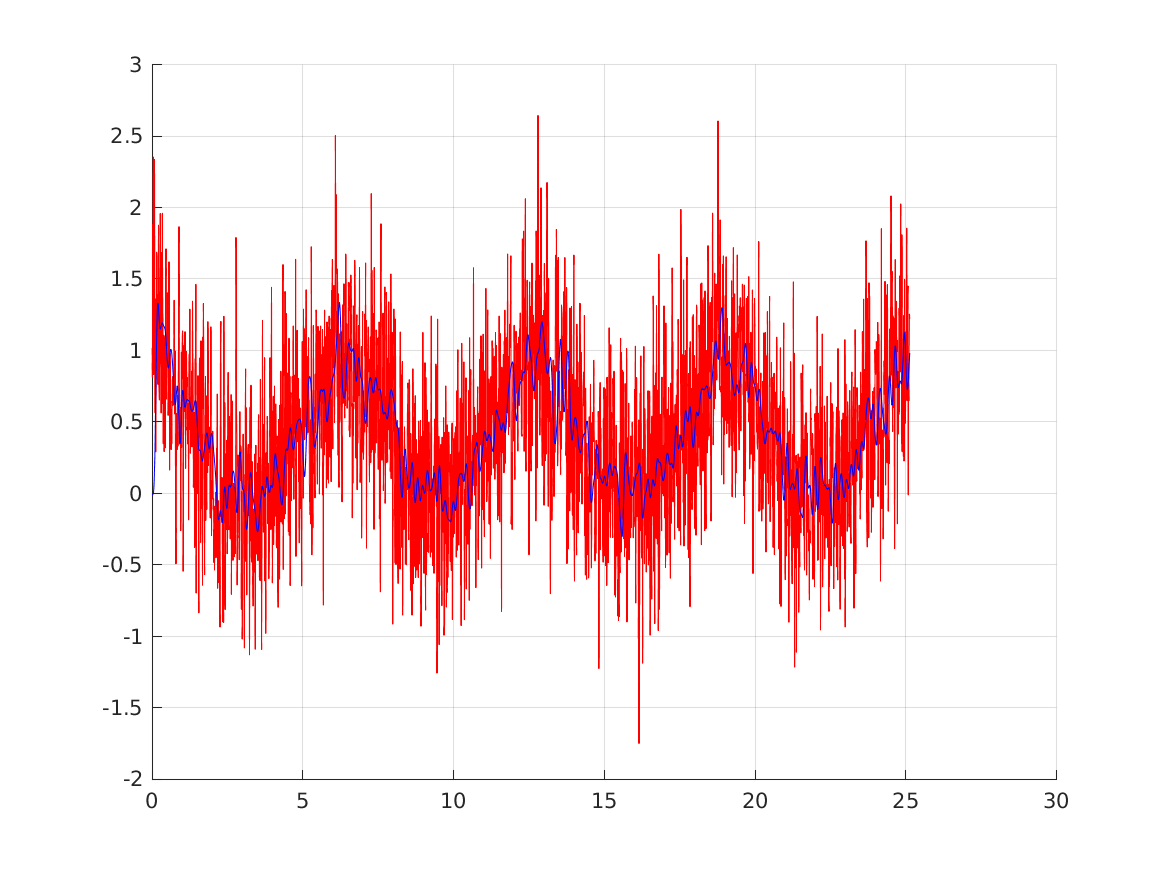
\includegraphics[scale=0.7]{lab3/figures/figure_16.png}\\
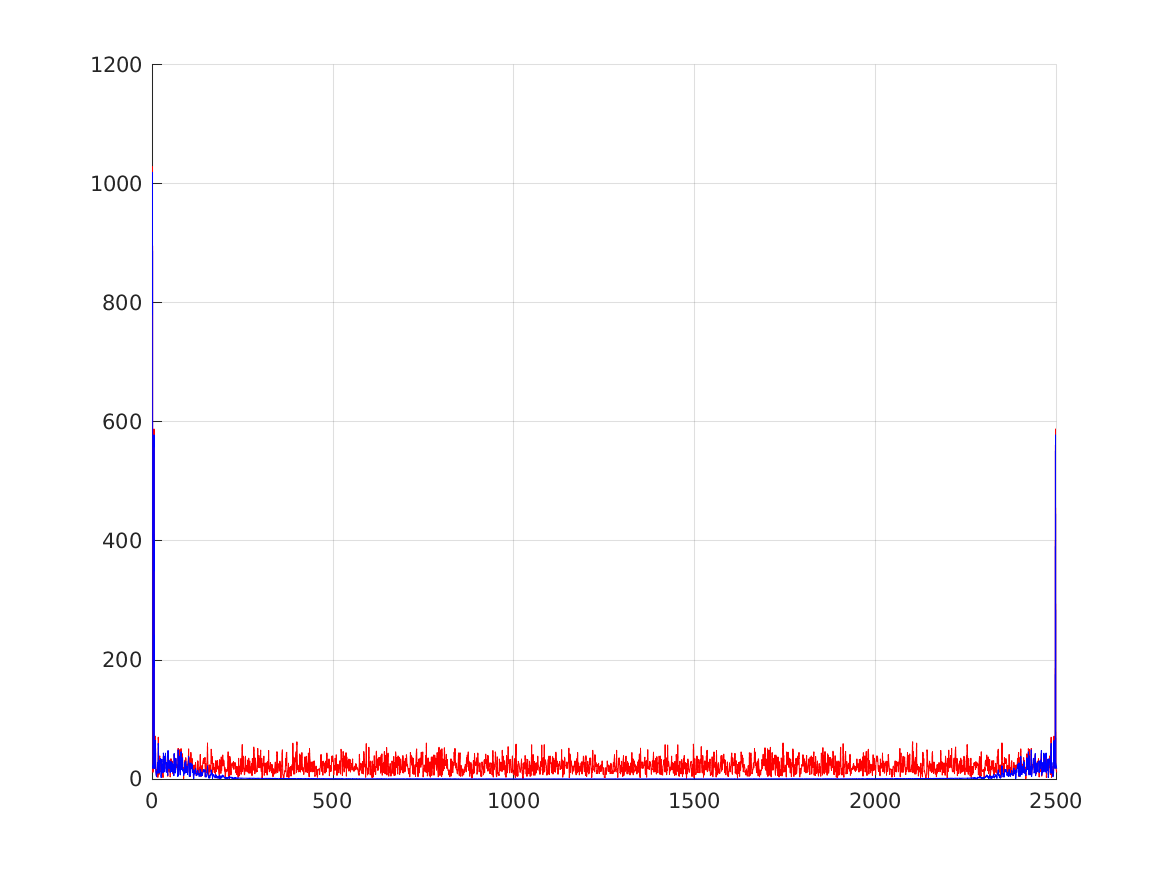
\includegraphics[scale=0.7]{lab3/figures/figure_17.png}\\
\section{Вывод}
В ходе данной работы было рассмотрено восстановление зашумленных сигналов с помощью линейного фильтра. В результате фильтрации часть высокочастотных шумов исчезла. В результате на выходе мы наблюдали частично восстановленный гармонический сигнал.
Причина неполного удаления шума линейным фильтром в том, что белый шум имеет сплошной спектр, из чего следует, что он попадет в полосу пропускания фильтра. Из-за этого мы наблюдаем на выходе гармонический сигнал не полностью восстановленный, а слегка с искажениями.
\end{document}